\section{RIA Application}

Our RIA application was created using the Java Applet Library. It features two main functionality: Signing a file and verifying a signed file. To sign a file, the user requires a file to be signed, a private key file, and the pass phrase for the private key. The signed file will be outputted to the same location as the input file. To verify the file, the user requires the original file, the signed file, and the public key. Features that our RIA include are:

\begin{itemize}
    \item File dialog for selecting files
    \item Text input field for pass phrase
    \item Basic menu interface, with back options
    \item Changing button text colour upon selecting a file (red to green)
    \item Error messages
    \item Success messages 
    \item Unexpected input handling
\end{itemize}

\subsection{UI Design}

\begin{figure}[hbt!]
	\centering
      
\includegraphics[width=0.6\textwidth]{imgs/ria/main} \\
	\caption{Main Menu}
	\label{fig:specifiyingkeysize}
    \noindent\makebox[\linewidth]{}
\end{figure}

\begin{figure}[hbt!]
	\centering
      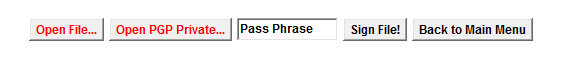
\includegraphics[width=0.6\textwidth]{imgs/ria/sign} \\
	\caption{Sign File - Nothing Selected}
	\label{fig:specifiyingkeysize}
    \noindent\makebox[\linewidth]{}
\end{figure}

\begin{figure}[hbt!]
	\centering
      
\includegraphics[width=0.6\textwidth]{imgs/ria/sdigngreen} \\
	\caption{Sign File - Files Selected}
	\label{fig:specifiyingkeysize}
    \noindent\makebox[\linewidth]{}
\end{figure}

\begin{figure}[hbt!]
	\centering
      
\includegraphics[width=0.6\textwidth]{imgs/ria/successsign} \\
	\caption{Sign File - Success}
	\label{fig:specifiyingkeysize}
    \noindent\makebox[\linewidth]{}
\end{figure}

\begin{figure}[hbt!]
	\centering
      
\includegraphics[width=0.6\textwidth]{imgs/ria/error} \\
	\caption{Sign File - Error}
	\label{fig:specifiyingkeysize}
    \noindent\makebox[\linewidth]{}
\end{figure}

\begin{figure}[hbt!]
	\centering
      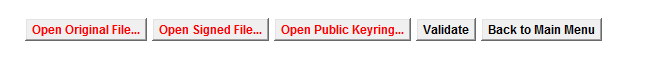
\includegraphics[width=0.6\textwidth]{imgs/ria/verifyred} \\
	\caption{Verify File - Nothing Selected}
	\label{fig:specifiyingkeysize}
    \noindent\makebox[\linewidth]{}
\end{figure}

\begin{figure}[hbt!]
	\centering
      
\includegraphics[width=0.6\textwidth]{imgs/ria/verfygreen} \\
	\caption{Verify File - Files Selected}
	\label{fig:specifiyingkeysize}
    \noindent\makebox[\linewidth]{}
\end{figure}

\begin{figure}[hbt!]
	\centering
      
\includegraphics[width=0.6\textwidth]{imgs/ria/sucessverify} \\
	\caption{Verify File - Success}
	\label{fig:specifiyingkeysize}
    \noindent\makebox[\linewidth]{}
\end{figure}

\begin{figure}[hbt!]
	\centering
      
\includegraphics[width=0.6\textwidth]{imgs/ria/error2} \\
	\caption{Verify File - Error}
	\label{fig:specifiyingkeysize}
    \noindent\makebox[\linewidth]{}
\end{figure}


